\chapter{OpenTE: Open Transition System with Encapsulated State}
\label{ch:oe}

The previous chapter demonstrated how CompCertO semantics
can be extended with additional state
to support compositional verification.
This chapter further refines the treatment of state
by addressing a critical limitation:
while OpenTX enables compositional reasoning with external state,
it still requires clients to explicitly manage
the state of components they depend on.
By identifying common patterns in verification tasks,
this chapter introduces \emph{state encapsulation}
to reduce boilerplate proofs and enhance modularity.

A recurring pattern emerges in compositional verification:
a client module typically does not need
to understand the implementation details
of downstream modules it depends on.
However,
to ensure interface compatibility,
the client must be lifted with the state of downstream modules,
and the corresponding correctness proof
must be manually adapted
to account for this additional state.
State encapsulation streamlines this process
by allowing downstream modules
to hide their internal state from clients.
This allows the client to remain unaware of
the internal states of modules it depends on,
while the framework automatically manages
the underlying state transitions and their proofs.

Beyond state encapsulation,
this chapter introduces practical mechanisms
for implementing these theoretical advances.
Building on the memory separation techniques from the previous chapter,
a new language, $\kw{ClightP}$, is presented
that operates on memory states extended with an additional environment.
The environment serves as an intermediate abstraction layer
between abstract state and CompCertO memory fragments,
abstracting away low-level memory details
and simplifying abstraction relation definitions.
Compilation from $\kw{ClightP}$ to $\kw{Clight}$ automatically translates
the environment into memory fragments
and merges them with the main memory state via the frame rule.

\begin{table}
  \centering
  \begin{tabular}{ll}
    \toprule
    Notation & Description\\
    \midrule
    $w \sysstep w'$ & Accessibility Relation for the System (Def.~\ref{def:bg:sc})\\
    $w \mathbin{\color{red}{\envstep}} w'$ & Accessibility Relation for the Environment (Def.~\ref{def:oe:ssc})\\
    $\mathbb{R} : A \twoheadleftrightarrow B$ & (Overloaded) Stateful Simulation Convention (Def.~\ref{def:oe:ssc})\\
    $L_1 \preceq_{\mathbb{R} \twoheadrightarrow \mathbb{S}} L_2$ & Stateful Simulation between Ordinary Transition Systems (Def.~\ref{def:oe:ssim})\\
    $\langle u, L \rangle$ & Transition System with Encapsulated State (Def.~\ref{ox:def:ets})\\
    $L : A \twoheadrightarrow B$ & (Overloaded) Transition System with Encapsulated State (Def.~\ref{ox:def:ets})\\
    $L_1 \le_{\mathbb{R} \twoheadrightarrow \mathbb{S}} L_2$ & (Overloaded) Simulation between LTS with Encapsulation (Sec.~\ref{sec:oe:sim-encap})\\
    $f : U \lensarrow V$ & (Overloaded) Stateful Lens (Def.~\ref{oe:def:lens-stateful})\\
    $\encap{u}$ & Encapsulation Primitive (Def.~\ref{sec:oe:encap-primitive})\\
    $\kw{ClightP}(\kw{p.c})$ & ClightP Semantics\\
    $\kw{ClightP}\langle \kw{p.c} \rangle$ & ClightP Semantics with Persistent State Encapsulated\\
    \bottomrule
  \end{tabular}
  \caption{Summary of notations}
  \label{tab:oe:notations}
\end{table}

The remainder of this chapter is structured as follows.
Section~\ref{sec:oe:intro-persistent} provides a high-level overview of approaches to state encapsulation.
Section~\ref{sec:oe:encap} develops the notion of state encapsulation within transition systems.
Sections~\ref{sec:oe:sim} and \ref{sec:oe:sim-encap} examine how simulation operates over encapsulated transition systems.
As concrete applications, Section~\ref{sec:oe:clightp} introduces the ClightP semantics, and Section~\ref{sec:oe:cal} presents an implementation of CAL with state encapsulation.

Table~\ref{tab:oe:notations} summarizes the notations used in this chapter.
Some of these notations are overloaded,
as they extend existing ones
to more general contexts.

\section{Approaches to State Encapsulation}
\label{sec:oe:intro-persistent}

\subsection{Persistent State}
\label{sec:oe:persistent-state}

Consider a simple example:
a counter module $L_\kw{cnt}$,
which records the number of times it is invoked.
In the vanilla CompCertO semantics,
such a counter relies on an external state
supplied together with the incoming question.
This arises from the \textit{ephemeral} nature of the CompCertO transition system,
where each invocation is solely determined
by the current question and
is independent of any prior interactions.
From the environment's perspective,
the following observable trace reflects
the sequence of interactions
where the updated state is threaded through questions and answers:
\[
  L_\kw{cnt} :
  \mathbf{0} \twoheadrightarrow \C \at \mathbb{N} \quad\vDash\quad
  \kw{inc}()\at [c \mapsto 0] \ \cdot\  0\at [c \mapsto 1] \ \cdot\
  \kw{inc}()\at [c \mapsto 1] \ \cdot\  1\at [c \mapsto 2] \ \cdot\ \cdots
\]
Crucially, the external state is returned to the environment
as part of the answer,
and it is the client's responsibility to ensure that
this state is passed to the subsequent invocation unchanged.
Verifying this preservation of state must be done explicitly
for each client,
often resulting in repetitive proofs.

This ephemeral nature can be addressed by introducing
\textit{persistent} state---state that is retained across invocations---into the semantics.
For example, a version of the counter can be defined
with a persistent state of type $\mathbb{N}$
initialized to $0 \in \mathbb{N}$.
In this setting, the observable trace evolves naturally with each call,
and there is no need for the client to manage or propagate the state explicitly.
\[
  L'_\kw{cnt} :
  \mathbf{0} \twoheadrightarrow \C \quad\vDash\quad
  \kw{inc}()\ \cdot\  0\ \cdot\
  \kw{inc}()\ \cdot\  1\ \cdot\
  \kw{inc}()\ \cdot\  2\ \cdot\ \cdots
\]

% When a transition system $L : A \twoheadrightarrow B$
% performs an outgoing call in $A$,
% the internal state $s$ is preserved
% until an answer resumes the execution,
% but no state is preserved across incoming calls in~$B$.
% Each question $q \in B^\que$ initializes a fresh state $s$
% such that $q \mathrel{I} s$
% regardless of any previous calls. % made into $L$.

To allow a component to retain state across calls,
one possible solution is to modify the definition of transition systems
to include a persistent state $U$ with an initial value $u_0$.
The initial and final state predicates
\begin{equation} \label{eqn:psts}
  u_0 \in U
  \qquad
  I \subseteq U \times B^\que \times S
  \qquad
  F \subseteq S \times B^\ans \times U
\end{equation}
could then access and update this persistent state,
with the understanding that on the first activation,
$I$ would be passed the persistent state $u_0$,
and that the updated value produced by $F$
in the context of one activation
would be used to initialize the next one.

Fortunately,
the situation described above
can already be encoded in the existing model with minimal effort
by using the language interface $B \at U$:
a component with persistent state is defined as a tuple
$\langle u_0 \in U, L \rangle$
where
$L : A \twoheadrightarrow B \at U$.
The key idea behind implementing persistent state is to
\textit{reuse} the external state passed along with the questions and answers,
and to
\textit{enforce that the client does not alter the state}
it receives---ensuring that it is passed unchanged between calls.
As long as this discipline is maintained,
the effect of persistent state can be achieved
within the existing ephemeral semantics.
This idea forms the foundation of state encapsulation for transition systems,
which will be explored in detail in Section~\ref{sec:oe:encap}.

\subsection{Kripke World Transitions}
\label{sec:oe:intro-kripke}

While the encoding above enables persistent state within existing semantics,
it introduces new challenges for simulation proofs.
Persistent states that are intrinsic to the semantics
require fundamental changes to simulation conventions. In the original CompCertO simulation proofs,
each time the simulation encounters outgoing questions,
it freshly chooses a Kripke world to relate the questions (cf.~\autoref{fig:bg:simint}).
This approach works well for ephemeral semantics
but breaks down when components maintain persistent state.

% Recall that Kripke worlds have already been in use for the simulation proofs of
% CompCertO to express rely and guarantee conditions on the states. Particularly,
% in some CompCertO compilation passes, the Kripke worlds are instantiated to
% memory injections. Typically, the memory injection relates the answers must be
% non-increasing compared to the injection that relates the questions. The
% non-increasing is encoded as the accessibility condition of the world.

More specifically, in a simulation proof $L_1 \le_{\mathbb{R} \twoheadrightarrow
\mathbb{S}} L_2$, if the incoming questions are related by $S^\que$ at world
$w_s$, the outgoing answers must be related at the same world. This is reflected
as the arrow from $q$ to $r$ in the following diagram. Conversely, at the
position of making outgoing questions, the simulation proof chooses a world
$w_r$ to relate the questions, and it can assume that the answers are related at
the same world. This corresponds to the arrows from $m_1$ to $n_1$, $m_2$ to
$n_2$, and $m_k$ to $n_k$ in the following diagram.
\[
  \begin{tikzpicture}[baseline=(current bounding box.center)]
    \node (q) at (0,0) {$q$};
    \node at (0.5,0) {$\cdot$};
    \node (m1) at (1,0) {$m_1$};
    \node at (1.5,0) {$\cdot$};
    \node (n1) at (2,0) {$n_1$};
    \node at (2.5,0) {$\cdot$};
    \node (m2) at (3,0) {$m_2$};
    \node at (3.5,0) {$\cdot$};
    \node (n2) at (4,0) {$n_2$};
    \node (dots) at (5,0) {$\cdots$};
    \node (mk) at (6,0) {$m_k$};
    \node at (6.5,0) {$\cdot$};
    \node (nk) at (7,0) {$n_k$};
    \node at (7.5,0) {$\cdot$};
    \node (r) at (8,0) {$r$};

    \draw[{Latex}-, shorten <=2pt, shorten >=2pt] (q.north).. controls +(0.5cm, 0.7cm) and +(-0.5cm, 0.7cm) .. (r.north);
    %\draw[{Latex}-, out=15, in=165] (q.north east) to (r.north west);
    \draw[{Latex}-, bend left=30, shorten <=2pt, shorten >=2pt] (m1.north) to (n1.north);
    \draw[{Latex}-, bend left=30, shorten <=2pt, shorten >=2pt] (m2.north) to (n2.north);
    \draw[{Latex}-, bend left=30, shorten <=2pt, shorten >=2pt] (mk.north) to (nk.north);
  \end{tikzpicture}
\]

With persistent states, however, the choice of Kripke world must account for
the computation's history. For example, when simulating between
the ephemeral counter $L_\kw{cnt}$ and the persistent counter $L'_\kw{cnt}$,
the simulation must choose a sequence of Kripke worlds
that tracks the evolving state:
\begin{gather*}
  w_0 \Vdash \kw{inc}() \ R^\que\ \kw{inc}() \at [c \mapsto 0] \\
  w_1 \Vdash \kw{inc}() \ R^\que\ \kw{inc}() \at [c \mapsto 1] \\
  w_2 \Vdash \kw{inc}() \ R^\que\ \kw{inc}() \at [c \mapsto 2] \\
  \cdots
\end{gather*}
Each world must remember the number of counter invocations,
which must equal the external state value $c$ in the target program.
This enables simulation of the source-level program
that maintains persistent counting state.
In essence, the simulation itself must be stateful
to handle stateful transition systems.
The solution is to introduce
a cross-call Kripke world transition relation
that constrains the choice of subsequent worlds.
The transition corresponds the red arrow in the
following diagram:
\[
  \begin{tikzpicture}[baseline=(current bounding box.center)]
    \node (q) at (0,0) {$q$};
    \node at (0.5,0) {$\cdot$};
    \node (m1) at (1,0) {$m_1$};
    \node at (1.5,0) {$\cdot$};
    \node (n1) at (2,0) {$n_1$};
    \node at (2.5,0) {$\cdot$};
    \node (m2) at (3,0) {$m_2$};
    \node at (3.5,0) {$\cdot$};
    \node (n2) at (4,0) {$n_2$};
    \node (dots) at (5,0) {$\cdots$};
    \node (mk) at (6,0) {$m_k$};
    \node at (6.5,0) {$\cdot$};
    \node (nk) at (7,0) {$n_k$};
    \node at (7.5,0) {$\cdot$};
    \node (r) at (8,0) {$r$};

    \draw[{Latex}-, shorten <=2pt, shorten >=2pt] (q.north).. controls +(0.5cm, 0.7cm) and +(-0.5cm, 0.7cm) .. (r.north);
    %\draw[{Latex}-, out=15, in=165] (q.north east) to (r.north west);
    \draw[{Latex}-, bend left=30, shorten <=2pt, shorten >=2pt] (m1.north) to (n1.north);
    \draw[red, {Latex}-, bend left=30, shorten <=2pt, shorten >=2pt] (n1.north) to (m2.north);
    \draw[{Latex}-, bend left=30, shorten <=2pt, shorten >=2pt] (m2.north) to (n2.north);
    \draw[{Latex}-, bend left=30, shorten <=2pt, shorten >=2pt] (mk.north) to (nk.north);
  \end{tikzpicture}
\]

In particular, for the example of the counter, the cross-call Kripke world
transition is defined to be the identity relation, which means that the world
that relates the last round of answers must be the same as the world that relates
the next round of questions. This way, the simulation can remember the value
of the internalized counter state.

This will be elaborated in Section~\ref{sec:oe:sim}.

\section{State Encapsulation}
\label{sec:oe:encap}

Having established the motivation and high-level approach to state encapsulation, the formal development of the framework can now begin.

\subsection{Encapsulated Transition System}

A transition system $L_1 : B \twoheadrightarrow C$
can interact with
$L_2 : A \twoheadrightarrow B \at U$
as the composite $(L_1 \at U) \odot L_2 : A \twoheadrightarrow C \at U$.
This situation guarantees by construction that
$L_1$ cannot interfere with the state component of type $U$
used by $L_2$.
The approach to state encapsulation
is to force the environment to
interact with components in this manner.

\begin{definition}[Encapsulated Transition System]
  \label{ox:def:ets}
  An encapsulated transition system is defined as the tuple
  $\langle u \in U, L \rangle : A \twoheadrightarrow B$,
  which consists of
  \begin{itemize}
    \item a set of states $U$ with an initial state $u \in U$;
    \item an underlying transition system $L : A \twoheadrightarrow B \at U$.
  \end{itemize}
\end{definition}

The first time
$\langle u \in U, L \rangle : A \twoheadrightarrow B$
is activated by a question $q \in B^\que$,
%the state $u$ is adjoined to $q$ and
the underlying component $L$ is initialized using %the question
$q@u \in (B \at U)^\que$.
When $L$ terminates with an answer $r@u' \in (B \at U)^\ans$,
the component passes $r \in B^\ans$ on to the environment and
the new state $u'$ is set aside to be used with the next activation.
This is guaranteed by the following definition of composition.

\begin{definition}[Composition of Encapsulated Transition Systems]
  \label{ox:def:ets-comp}
  Encapsulated transition systems have an identity component $\langle * \in
  \{*\}, \kw{id} : A \twoheadrightarrow A \rangle$, and compose as follows:
  \[
    \langle u \in U, L_1 \in B \twoheadrightarrow C \at U \rangle
    \odot
    \langle v \in V, L_2 \in A \twoheadrightarrow B \at V \rangle
    \::=\:
    \big\langle (u, v) \in U \times V, L_1 \at V \odot L_2 \big\rangle
  \]
  The composition of encapsulated transition systems is associative
  and admits the identity encapsulated transition system as units.
  In other words,
  encapsulated transition systems form a category $\mathbf{ETS}$.
\end{definition}

Note that the signature isomorphisms such as $A \cong A \at \{*\}$ and $A \at U
\at V \cong A \at (U \times V)$ are implicitly applied as usual.

\begin{example}
  \label{compceroe:ex:cnt}

  Consider a transition system $L_\kw{cnt} : \mathbf{0} \twoheadrightarrow \C
  \at \mathbb{N}$ that implements a simple counter. The counter yields the
  following trace from the view of the client:
  \[
    \kw{inc}()\at [c \mapsto 0] \ \cdot\  0\at [c \mapsto 1] \ \cdot\
    \kw{inc}()\at [c \mapsto 1] \ \cdot\  1\at [c \mapsto 2] \ \cdot\ \cdots
  \]
  Note that state cannot be maintained across calls with vanilla transition
  systems, so the counter keeps counting by mutating the state passed from the
  environment.

  The encapsulated transition system $\langle 0, L_\kw{cnt} \rangle : \mathbf{0}
  \twoheadrightarrow \C$ hides the extra state from the interaction boundaries,
  and associates the initial value $0$ with it, yielding the following trace:
  \[
    \kw{inc}() \cdot 0 \ \cdot\
    \kw{inc}() \cdot 1 \ \cdot\
    \kw{inc}() \cdot 2 \ \cdot\ \cdots
  \]
\end{example}

A regular transition system $L$
has a canonical embedding $\langle * \in \mathbf{1}, L \rangle$
that encapsulates the trivial state $\mathbf{1}$.
The embedding is functorial in that it preserves the identity and composition.

Notation-wise,
$L : A \twoheadrightarrow B$ is overloaded
to denote an encapsulated transition system
and $|L|$ is written for the underlying transition system.
In cases where it is ambiguous
whether $L : A \twoheadrightarrow B$ refers to a regular or encapsulated transition system,
it defaults to interpreting it as encapsulated,
since any regular transition system can be canonically lifted to an encapsulated one.

\subsection{Stateful Lenses}

Recall that a lens
can be viewed as a passive transition system (see \S\ref{sec:ox:lens}).
Thus,
the approach to persistent state
can be applied to lenses as well
to obtain \textit{stateful lenses}.

\begin{definition}
  \label{oe:def:lens-stateful}
  A \emph{stateful lens} between the sets $U$ and $V$,
  written $f : U \leftrightarrows V$,
  is given by a set $P$ of \emph{persistent states},
  an \emph{initial state} $p_0 \in P$,
  and an underlying lens $|f| : U \leftrightarrows V \times P$.

  The identity lens $\kw{id}_U : U \leftrightarrows U$
  uses the singleton set $\{*\}$ as its persistent state and is defined by:
  \[
    \kw{get}_{\kw{id}_U}(u, *) := u
    \,,
    \qquad
    \kw{set}_{\kw{id}_U}(u, *, u') := (u', *)
    \,.
  \]
  The composite $g \circ f$ of
  $f : U \leftrightarrows V$ and
  $g : V \leftrightarrows W$
  uses pairs of persistent states of $f$ and $g$ and
  is described by:
  \begin{gather*}
    \kw{get}_{g \circ f}(w, p, q) := \kw{get}_f(\kw{get}_g(w, p), q)
    \,,
    \\[1.5ex]
    \begin{prooftree}
      \hypo{\kw{get}_f(w, p) = v}
      \hypo{\kw{set}_g(v, q, u) = (v', q')}
      \hypo{\kw{set}_f(w, p, v') = (w', p')}
      \infer3{\kw{set}_{g \circ f}(w, p, q, u) = (w', p', q') \,.}
    \end{prooftree}
  \end{gather*}
\end{definition}

\begin{theorem}[Properties of Stateful Lens Composition]
  The composition of stateful lenses is associative
  and admits identity lenses as units.
\end{theorem}

Stateful lenses
are embedded into encapsulated transition systems
by applying the embedding defined in Definition \ref{ox:def:lts-lens}
to the underlying lens.
\[
  \llbracket \langle p_0 \in P, f \rangle : U \leftrightarrows V \rrbracket
  \::=\:
  \langle p_0 \in P, \llbracket f \rrbracket \rangle : [U] \twoheadrightarrow [V]
\]

\subsection{Encapsulation Primitives}
\label{sec:oe:encap-primitive}

The stateful lens that is particularly useful
is the \emph{encapsulation primitive},
which can be used to turn
an explicit state component into a private one.
\[
  \encap{u} : U \leftrightarrows \mathbf{1} \::=\: \langle u \in U, \kw{id}_U \rangle
\]
This primitive uses $U$ for its persistent state.
When it is activated by $* \in \{*\}$,
the current state (initially $u \in U$)
is used as an outgoing question;
the answer $u' \in U$ is then used as an updated state for the next activation.

\begin{example}
  Using the encapsulation primitive,
  the encapsulated counter can be alternatively defined as
  \[
    (\kw{id}_\C \at \encap{0}) \odot L_\kw{cnt} : \mathbf{0} \twoheadrightarrow \C
  \]
  where $L_\kw{cnt}$ is implicitly embedded into the canonical encapsulated transition system.
  This definition is equivalent to the one in Example~\ref{compceroe:ex:cnt}.
  The use of the encapsulation primitive
  allows the simulation proof to be decomposed into
  smaller, modular components,
  making it possible to reuse the correctness proofs
  for the non-encapsulated part.
  This will be elaborated on in \S\ref{sec:oe:repr}.
\end{example}

As discussed in \S\ref{sec:ox:lens},
the behavior of the lens $\encap{u}$,
viewed as a transition system,
is non-deterministic.
Composing with the active component
$\kw{id}$---which transparently forwards questions and answers---%
the overall behavior conforms to the structure of $\kw{id}$,
with state properly encapsulated.
This is depicted in the following diagram.

\[
  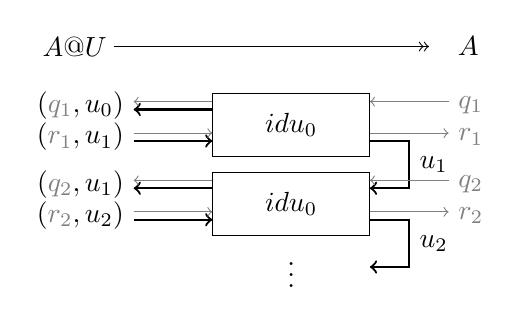
\begin{tikzpicture}[yscale=0.2,xscale=0.5]
    \begin{scope}
      \draw[fill=white] (0,0) rectangle (4,4) node[midway] {$\kw{id} \at \encap{u_0}$};
      \draw[fill=white] (0,5) rectangle (4,9) node[midway] {$\kw{id} \at \encap{u_0}$};
    \end{scope}
    \begin{scope}[thick]
      \draw[->] (0,8) -- (-2,8); % outgoing u0
      \draw[->] (-2,6) -- (0,6); % incoming u1
      \draw[->] (0,3) -- (-2,3); % outgoing u1
      \draw[->] (-2,1) -- (0,1); % incoming u2
    \end{scope}
    \begin{scope}[thick]
      \draw[->] (4,6) -- (5,6) -- node[right] {$u_1$} (5,3) -- (4,3);
      \draw[->] (4,1) -- (5,1) -- node[right] {$u_2$} (5,-2) -- (4,-2);
    \end{scope}
    \begin{scope}[yshift=0.25cm]
      \draw (6,8) node[right] {$\textcolor{gray}{q_1}$};
      \draw (-2,8) node[left] {$(\textcolor{gray}{q_1}, u_0)$};
      \draw (-2,6) node[left] {$(\textcolor{gray}{r_1}, u_1)$};
      \draw (6,6) node[right] {$\textcolor{gray}{r_1}$};
      \draw (6,3) node[right] {$\textcolor{gray}{q_2}$};
      \draw (-2,3) node[left] {$(\textcolor{gray}{q_2}, u_1)$};
      \draw (-2,1) node[left] {$(\textcolor{gray}{r_2}, u_2)$};
      \draw (6,1) node[right] {$\textcolor{gray}{r_2}$};
    \end{scope}
    \begin{scope}[gray,yshift=0.5cm]
      \draw[->] (6,8) -- (4,8); % incoming q1
      \draw[->] (0,8) -- (-2,8); % outgoing q1
      \draw[->] (-2,6) -- (0,6); % incoming r1
      \draw[->] (4,6) -- (6,6); % outgoing r1
      \draw[->] (6,3) -- (4,3); % incoming q2
      \draw[->] (0,3) -- (-2,3); % outgoing q2
      \draw[->] (-2,1) -- (0,1); % incoming r2
      \draw[->] (4,1) -- (6,1); % outgoing r2
    \end{scope}
    \begin{scope}
      \node at (2,-2) {$\vdots$};
      \node at (-3.5,12) {$A@U$};
      \node at (6.5,12) {$A$};
      \draw[->>] (-2.5,12) -- (5.5,12);
    \end{scope}
  \end{tikzpicture}
\]

\begin{example} \label{ex:encaps-bq}
  The component
  $\Gamma_\kw{bq} :=
  \bigl(\kw{id}_\C \at \encap{\epsilon}\bigr) \odot L_\kw{bq} :
  \mathbf{0} \twoheadrightarrow \C$
  describes the behavior of an initially empty bounded queue.
  The set of abstract states $D_\kw{bq}$ is used to define it,
  but is not exposed as part of its interface,
  so that client code will only observe call traces
  where state is implicit:
  \[
    \Gamma_\kw{bq} \: \vDash \:
    (\kw{enq}[v_1] \rightarrowtail {*}) \leadsto
    (\kw{enq}[v_2] \rightarrowtail {*}) \leadsto
    (\kw{deq} \rightarrowtail v_1) \leadsto
    (\kw{enq}[v_3] \rightarrowtail {*}) \leadsto
    (\kw{deq} \rightarrowtail v_2) \leadsto \cdots
  \]
  Likewise,
  $d_0 := (\{\ldots\}, 0, 0) \in D_\kw{rb}$
  can be used to define
  $\Gamma_\kw{rb} :=
  \bigl( \kw{id}_\C \at \encap{d_0} \bigr) \odot L_\kw{rb} :
  \mathbf{0} \twoheadrightarrow \C$
  as an encapsulated specification for
  the ring buffer data structure.
\end{example}

\section{Stateful Simulation}
\label{sec:oe:sim}

In this section,
I will provide a formal definition of stateful simulation conventions
and show how to adapt the simulation conditions to account for the cross-call
Kripke world transition.

\subsection{Stateful Simulation Convention}

Simulation conventions characterize the relationship between source- and
target-level questions and answers.
In CompCertO, each pair of calls is related
in isolation,
without reference to past or future calls.
This notion is generalized to allow invariants on states
to be maintained across calls.
To this end,
the definition is extended
to incorporate both an initial world
and the world transition across calls.

\begin{definition}
  \label{def:oe:ssc}
  A stateful simulation convention
  $\mathbb{R} = \langle W, w_0, \red{\envstep}, \sysstep, R^\que, R^\ans \rangle : A \twoheadleftrightarrow B$
  is specified by:
  \begin{itemize}
    \item a set $W$ of worlds with an initial world $w_0 \in W$;
    \item an environment accessibility relation $\red{\envstep} \:\subseteq\: W \times W$;
    \item a system accessibility relation $\sysstep \:\subseteq\: W \times W$;
    \item a Kripke question relation $R^\que \:\subseteq\: \mathcal{R}_W(A^\que, W)$;
    \item a Kripke answer relation $R^\ans \:\subseteq\: \mathcal{R}_W(A^\ans, W)$.
  \end{itemize}
  The accessibility relations are required to be reflexive and transitive.
\end{definition}

The initial world $w_0$ gives the simulation convention's initial state.
While the environment is in control,
the world may transition according to the relation $\red{\envstep}$.
When control is transferred to the system,
the corresponding questions must be related by $w \Vdash R^\que$.
World transitions may then occur according to $\sysstep$.
Hence, when the system returns control to the environment,
the corresponding answers
will be related by $w' \Vdash R^\ans$,
where $w'$ is a successor world of $w$ such that $w \sysstep w'$.
The questions for any subsequent activation
must in turn be related at a world $w''$ such that $w' \mathbin{\red{\envstep}} w''$,
and so on and so forth indefinitely:
\begin{align*}
  w_0 \mathbin{\red{\envstep}} w_1 &\Vdash q_1 \mathrel{R^\que} q'_1 \\
  w_1 \sysstep w_1' &\Vdash r_1 \mathrel{R^\ans} r'_1 \\
  w_1' \mathbin{\red{\envstep}} w_2 &\Vdash q_2 \mathrel{R^\que} q'_2 \\
  w_2 \sysstep w_2' &\Vdash r_2 \mathrel{R^\ans} r'_2 \\[-1ex]
  &\:\:\vdots
\end{align*}

The example below illustrates this idea
in a simple setting,
where the world tracks the value of a counter
and the system may update it
while the environment must leave it unchanged.
This demonstrates
how the world component
enforces cross-call invariants in practice.

\begin{example}
  \label{compceroe:ex:sc}
  Referring back to the example in \autoref{sec:oe:intro-kripke},
  the following simulation convention
  can relate the source-level behavior
  where the counter is encapsulated
  and the target-level behavior
  where the counter is explicitly passed:
  \begin{gather*}
    \mathbb{R} : \C \twoheadleftrightarrow \C \at \mathbb{N} :=
    \langle \mathbb{N}, 0, \red{=}, \top, R^\que, R^\ans \rangle
    \\
    \begin{prooftree}
      \infer0{n \Vdash \kw{inc}() \:R^\que\: \kw{inc}() \at [c \mapsto n]}
    \end{prooftree}
    \qquad
    \begin{prooftree}
      \infer0{n + 1 \Vdash \kw{inc}() \:R^\ans\: \kw{inc}() \at [c \mapsto n+1]}
    \end{prooftree}
  \end{gather*}
  where the notation $\top = \mathbb{N} \times \mathbb{N}$ is the total
  relation.
\end{example}

Next, I will define how stateful simulation conventions compose.
Just as ordinary simulation conventions
can be combined to relate multi-stage transformations,
stateful conventions can be composed
while preserving their world structure.

\begin{definition}[Composition of stateful simulation conventions]
  \label{ox:def:ssc-comp}
  The identity simulation convention $\mathbf{id}_A: A \twoheadleftrightarrow A$ is
  given by:
  \[
    \mathbf{id}_A = \langle \mathbf{1}, *, \red{=_\mathbf{1}},
    =_\{*\}, =_{A^\que}, =_{A^\ans} \rangle .
  \]
  The simulation convention
  $\mathbb{R}_1 : A \twoheadleftrightarrow B$ and
  $\mathbb{R}_2 : B \twoheadleftrightarrow C$ compose into
  $\mathbb{R}_1 \mathbin\fatsemi \mathbb{R}_2 : A \twoheadleftrightarrow C$,
  which is defined with the following components:
  \begin{align*}
    W &:= W_1 \times W_2 &
    R^\que & : R^\que_1 \times R^\que_2 &
    (w_1, w_2) \:\red{\envstep}\: (w'_1, w'_2) &\::\Leftrightarrow\:
    w_1 \:\red{\envstep}_1\: w'_1 \land w_2 \:\red{\envstep}_2\: w'_2 \\
    w_0 &:= (w^1_0, w^2_0) &
    R^\ans & : R^\ans_1 \times R^\ans_2 &
    (w_1, w_2) \:\sysstep\: (w'_1, w'_2) &\::\Leftrightarrow\:
    w_1 \:\sysstep_1\: w'_1 \land w_2 \:\sysstep_2\: w'_2
  \end{align*}
  The composition is associative
  and admits the identity simulation convention as units.
  In other words,
  stateful simulation conventions form a category $\mathbf{SSC}$.
\end{definition}

Finally, to connect this generalized notion
back to the familiar setting,
it is observed that
any regular simulation convention
can be canonically embedded into a stateful one.
This is done
by introducing a trivial initial world
and leaving the environment accessibility relation unrestricted.

\begin{definition}
  Given a regular simulation convention
  $\mathbb{R} : A \twoheadleftrightarrow B = \langle W, \sysstep, R^\que, R^\ans \rangle$,
  its stateful embedding is given by
  $
  \langle
  W \cup \{*\},
  *,
  \red{\top},
  \sysstep,
  R^\que,
  R^\ans
  \rangle
  $,
  where $\top$ is the total relation.
\end{definition}
This embedding allows the same notation $\mathbb{R} : A \twoheadleftrightarrow B$
to be used for both regular and stateful conventions,
defaulting to the stateful interpretation
when context does not specify otherwise.

\subsection{Stateful Simulation}

I can now define the generalized notion of simulation.%
\footnote{
  I will again omit some details
  which the model retains,
  such as CompCert's approach to
  demonic nondeterminism,
  silent divergence,
  and termination preservation,
  but which do not present any particular difficulty.
}
Consider a simulation
$
%\begin{tikzcd}
%  A_1 \ar[r, twoheadrightarrow, "L_1"] \ar[d, leftrightarrow, "\mathbf{R}_A"'] &
%  B_1 \ar[d, leftrightarrow, "\mathbf{R}_B"] \\
%  A_2 \ar[r, twoheadrightarrow, "L_2"] & B_2
%\end{tikzcd}
\phi : L_1 \le_{\mathbb{R}_A \twoheadrightarrow \mathbb{R}_B} L_2
$.

The simulation simultaneously
plays the role of the environment ($\red{\envstep}$) with respect to
the simulation convention $\mathbb{R}_A : A_1 \twoheadrightarrow A_2$ and
the role of the system ($\sysstep$) with respect to $\mathbb{R}_B : B_1 \twoheadrightarrow B_2$.
Hence,
it will operate in the context of a Kripke frame
constructed from both $W_A$ and $W_B$.
The possible states of a simulation will be a subset
$W \subseteq W_A \times W_B$,
which must contain
the pair of initial worlds.
Between successive activations,
the environment may update the $W_B$ component.
Hence it is required that:
\[
  (w_A, w_B) \in W \:\wedge\:
  w_B \mathbin{\red{\envstep}} w_B' \:\Rightarrow\:
  (w_A, w_B') \in W
\]
Conversely, for external calls,
the simulation plays the role of the environment.
It is expected that:
\[
  (w_A, w_B) \in W \:\wedge\:
  w_A \mathbin{\red{\envstep}} w_A' \:\Rightarrow\:
  (w_A', w_B) \in W
\]

When the components execute,
the worlds will evolve
from $(w_A, w_B)$ to $(w_A', w'_B)$
according to
the following accessibility relation.
This is used to formulate the conditions (a), (b), and (c) of \autoref{fig:oe:simint}:
\[
  w_A \mathbin{\red{\envstep}} w_A' \:\wedge\: w_B \sysstep w_B'
\]

% \begin{figure}
%   \small
%   \[
%     \begin{array}{c@{\qquad}c@{\qquad}c}
%       \begin{tikzcd}[sep=tiny,column sep=0]
%         q_1 \ar[dd, "w \Vdash \mathbf{R}_B^\que"', dash] \ar[rr, dash, "I_1"] &&
%         s_1 \ar[dd, "w' \Vdash R", dash, dashed] \\
%         & \leadsto_{\bar{A}B} & \\
%         q_2 \ar[rr, "I_2"', dash, dashed] &&
%         s_2
%       \end{tikzcd}
%       &
%       \begin{tikzcd}[sep=tiny,column sep=0]
%         s_1 \ar[rr, "t"] \ar[dd, "w \Vdash R"', dash] &&
%         \!\!{}_1 \:\, s_1' \ar[dd, "w' \Vdash R", dash, dashed] \\
%         & \leadsto_{\bar{A}B} & \\
%         s_2 \ar[rr, "t", dashed] &&
%         \!\!{}_2^* \:\, s_2'
%       \end{tikzcd}
%       %      \begin{tikzcd}[sep=large]
%       %        s_1 \ar[r] \ar[d, "{(w_A, w_B) \Vdash R}"', dash] &
%       %        s_1' \ar[d, "{(w_A,w_B) \Vdash R}", dash, dashed] \\
%       %        s_2 \ar[r, dashed] &
%       %        \!\!\!{}^* \: s_2'
%       %      \end{tikzcd}
%       &
%       \begin{tikzcd}[sep=tiny, column sep=0]
%         s_1 \ar[rr, "F_1", dash] \ar[dd, "w \Vdash R"', dash] &&
%         r_1 \ar[dd, "w' \Vdash \mathbf{R}_B^\ans", dash, dashed] \\
%         & \leadsto_{\bar{A}B} & \\
%         s_2 \ar[rr, "F_2"', dash, dashed] &&
%         r_2
%       \end{tikzcd}
%       \vspace{1ex} \\
%       I_1 \ifr{\Vdash \mathbf{R}_B^\que \rightarrow
%       \mathcal{P}^\le(\Diamond_{\bar{A}B} R)} I_2
%       &
%       {\rightarrow_1}
%       \ifr{\Vdash R \rightarrow \mathcal{P}^\le(\Diamond_{\bar{A}B} R)}
%       {\rightarrow_2^*}
%       &
%       F_1
%       \ifr{\Vdash R \rightarrow \mathcal{P}^\le(\Diamond_{\bar{A}B} \mathbf{R}_B^\ans)}
%       F_2
%       \vspace{1.2ex} \\
%       \text{(a) Initial states} &
%       \text{(b) Internal states} &
%       \text{(c) Final states}
%     \end{array}
%   \]
%   \[
%     \begin{array}{c}
%       \begin{tikzcd}[sep=tiny, column sep=small]
%         s_1 \ar[rr, "X_1", dash] \ar[dd, "w \Vdash R"', dash] &&
%         m_1 \ar[rr, dotted, dash] \ar[dd, "w'"', "{} \Vdash \mathbf{R}_A^\que", dash, dashed] &&
%         n_1 \ar[rr, "Y_1^{s_1}", dash] \ar[dd, "w''"', "{} \Vdash \mathbf{R}_A^\ans", dash] &&
%         s_1' \ar[dd, "w''' \Vdash R", dash, dashed]
%         \\
%         & \leadsto_{\bar{A}B} && \leadsto_{AB} && \leadsto_{\bar{A}B} &
%         \\
%         s_2 \ar[rr, "X_2"', dash, dashed] &&
%         m_2 \ar[rr, dotted, dash] &&
%         n_2 \ar[rr, "Y_2^{s_2}"', dash, dashed] &&
%         s_2'
%       \end{tikzcd}
%       \vspace{1ex} \\
%       Z_1
%       \mathrel{[
%           \Vdash R \rightarrow \mathcal{P}^\le(
%             \Diamond_{\bar{A}B} (
%               \mathbf{R}_A^\que \times
%               \Box_{AB} (
%                 \mathbf{R}_A^\ans \rightarrow
%           \mathcal{P}^\le(\Diamond_{\bar{A}B} R))))
%       ]}
%       Z_2
%       \vspace{1.3ex} \\
%       \text{(d) Outgoing calls}
%     \end{array}
%   \]

%   \caption{Stateful simulation properties for internal steps (a,b,c)
%   and outgoing calls (d).}
%   \label{fig:simint}
% \end{figure}

\begin{figure}
  \small
  \[
    \begin{array}{c@{\qquad}c@{\qquad}c}
      \begin{tikzcd}[row sep=3.5ex, column sep=3.5ex]
        q_1 \ar[dd, "w_B \Vdash \mathbb{R}_B^\que"', dash] \ar[rr, dash, "I_1"] &&
        s_1 \ar[dd, "w'_A{,} w'_B \Vdash R", dash, dashed] \\
        && \\
        q_2 \ar[rr, "I_2"', dash, dashed] &&
        s_2
      \end{tikzcd}
      &
      \begin{tikzcd}[row sep=3.5ex, column sep=3.5ex]
        s_1 \ar[rr] \ar[dd, "w_A{,} w_B \Vdash R"', dash] &&
        \!\!{}_1 \:\, s_1' \ar[dd, "w'_A{,} w_B' \Vdash R", dash, dashed] \\
        && \\
        s_2 \ar[rr, dashed] &&
        \!\!{}_2^* \:\, s_2'
      \end{tikzcd}
      %      \begin{tikzcd}[sep=large]
      %        s_1 \ar[r] \ar[d, "{(w_A, w_B) \Vdash R}"', dash] &
      %        s_1' \ar[d, "{(w_A,w_B) \Vdash R}", dash, dashed] \\
      %        s_2 \ar[r, dashed] &
      %        \!\!\!{}^* \: s_2'
      %      \end{tikzcd}
      &
      \begin{tikzcd}[row sep=3.5ex, column sep=3.5ex]
        s_1 \ar[rr, "F_1", dash] \ar[dd, "w_A{,} w_B \Vdash R"', dash] &&
        r_1 \ar[dd, "w_B' \Vdash \mathbb{R}_B^\ans", dash, dashed] \\
        && \\
        s_2 \ar[rr, "F_2"', dash, dashed] &&
        r_2
      \end{tikzcd}
      \vspace{1.2ex} \\
      \text{(a) Initial states} &
      \text{(b) Internal states} &
      \text{(c) Final states}
    \end{array}
  \]
  \[
    \begin{array}{c}
      \begin{tikzcd}[row sep=4.5ex, column sep=4.5ex]
        s_1 \ar[rr, "X_1", dash] \ar[dd, "w_B \Vdash R"', dash] &&
        m_1 \ar[rr, dotted, dash] \ar[dd, "w'_A"', "{} \Vdash \mathbb{R}_A^\que", dash, dashed] &&
        n_1 \ar[rr, "Y_1^{s_1}", dash] \ar[dd, "w''_A"', "{} \Vdash \mathbb{R}_A^\ans", dash] &&
        s_1' \ar[dd, "w'''_A{,} w_B' \Vdash R", dash, dashed]
        \\
        &&
        \\
        s_2 \ar[rr, "X_2"', dash, dashed] &&
        m_2 \ar[rr, dotted, dash] &&
        n_2 \ar[rr, "Y_2^{s_2}"', dash, dashed] &&
        s_2'
      \end{tikzcd}
      \vspace{1ex} \\
      \text{(d) Outgoing calls}
    \end{array}
  \]
  \vspace{1.5ex}
  \[
    \begin{array}{c@{\qquad}l}
      \vspace{2.8ex}
      (a) &
      {
        \begin{aligned}
          \forall\; w_A, w_B, q_1, q_2, s_1 .\;
          & q_1 \xrightarrow{I_1} s_1
          \:\wedge\:
          w_B \Vdash q_1 \mathbin{\mathbb{R}_B^\que} q_2 \:\Rightarrow
          \\
          \exists\; w'_A, w'_B, s_2.\;
          & q_2 \xrightarrow{I_2} s_2
          \:\wedge\:
          w_A \mathbin{\red{\envstep}} w'_A
          \:\wedge\:
          w_B \sysstep w'_B
          \:\wedge\:
          w'_A, w'_B \Vdash s_1 \mathbin{R} s_2
        \end{aligned}
      }
      \\
      \vspace{2.8ex}
      (b) &
      {
        \begin{aligned}
          \forall\; w_A, w_B, s_1, s_2, s_1' .\;
          & s_1 \rightarrow_1 s_1'
          \:\wedge\:
          w_A, w_B \Vdash s_1 \mathbin{R} s_2 \:\Rightarrow \\
          \exists\; w'_A, w'_B, s_2.\;
          & \bigl(s_2 \rightarrow^+_2 s_2'
            \:\vee\:
            s_2 \rightarrow^*_2 s_2'
            \:\wedge\:
            s_2' \le s_2
          \bigr) \:\wedge\: \\
          & w_A \mathbin{\red{\envstep}} w'_A
          \:\wedge\:
          w_B \sysstep w'_B
          \:\wedge\:
          w'_B \Vdash s_1' \mathbin{R} s_2'
        \end{aligned}
      }
      \\
      \vspace{2.8ex}
      (c) &
      {
        \begin{aligned}
          \forall\; w_A, w_B, s_1, s_2, r_1 .\;
          & s_1 \xrightarrow{F_1} r_1
          \:\wedge\:
          w_A, w_B \Vdash s_1 \mathbin{R} s_2 \:\Rightarrow \\
          \exists\; w'_A, w'_B, r_2.\;
          & r_1 \xrightarrow{F_2} r_2
          \:\wedge\:
          w_B \sysstep w'_B
          \:\wedge\:
          w'_B \Vdash r_1 \mathbin{\mathbb{R}_B^\ans} r_2
        \end{aligned}
      }
      \\
      (d) &
      {
        \begin{aligned}
          \forall\; w_A, w_B, s_1, s_2, m_1 .\;
          & s_1 \xrightarrow{X_1} m_1
          \:\wedge\:
          w_A, w_B \Vdash s_1 \mathbin{R} s_2
          \:\Rightarrow \\
          \exists\; w'_A, m_2.\;
          & s_2 \xrightarrow{X_2} m_2
          \:\wedge\:
          w_A \mathbin{\red{\envstep}} w'_A
          \:\wedge\:
          w'_A \Vdash m_1 \mathbin{\mathbb{R}_A^\que} m_2
          \:\wedge\: \\
          \forall\; w''_A, n_1, n_2, s_1'.\;
          & n_1 \xrightarrow{Y_1^{s_1}} s_1'
          \:\wedge\:
          w'_A \sysstep w''_A
          \:\wedge\:
          w''_A \Vdash n_1 \mathbin{\mathbb{R}_A^\ans} n_2
          \:\Rightarrow \\
          \exists\; w'''_A, w'_B, s'_2.\;
          & n_2 \xrightarrow{Y_2^{s_2}} s_2'
          \:\wedge\:
          w''_A \mathbin{\red{\envstep}} w'''_A
          \:\wedge\:
          w_B \sysstep w'_B
          \:\wedge\:
          w'''_A, w'_B \Vdash s_1' \mathbin{R} s_2'
        \end{aligned}
      }
    \end{array}
  \]
  \caption{Stateful simulation properties for internal steps (a,b,c)
  and outgoing calls (d).}
  \label{fig:oe:simint}
\end{figure}

Moreover,
from the point of view of the simulation,
when an external call is made,
the worlds will make a transition
from $(w_A, w_B)$ to $(w_A', w_B')$
according to
the following accessibility relation:
%[NB we may want to restrict $\leadsto_B$ to $=$
%if this causes problems, but]
%Note that by allowing a transition $w_B \leadsto_B w_B'$,
%we are able to capture the effect that
%any reentrant call may have on the simulation state:
\[
  w_A \sysstep w_A' \:\wedge\: w_B = w_B'
\]
$w_B$ is not updated
because the state is not passed
to the callee,
and reentrant calls are not allowed.
We can then formulate the simulation condition for external calls
as presented in condition (d) of \autoref{fig:oe:simint}.

\begin{definition}[Stateful open simulation]
  \label{def:oe:ssim}
  There is a simulation
  of $L_1 : A_1 \twoheadrightarrow B_1$
  by $L_2 : A_2 \twoheadrightarrow B_2$
  under the simulation conventions
  $\mathbb{R}_A : A_1 \twoheadleftrightarrow A_2$ and
  $\mathbb{R}_B : B_1 \twoheadleftrightarrow B_2$,
  if there exists
  \begin{itemize}
    \item a set of worlds $W$,
      closed under ${\leadsto_A} \times {\mapsto_B}$ and
      such that
      $(\intl{w}_A, \intl{w}_B) \in W \subseteq W_A \times W_B$;
      and
    \item
      a Kripke relation $R \in \mathcal{R}_W(S_1, S_2)$
      between the states of $L_1$ and $L_2$;
  \end{itemize}
  satisfying the properties given in
  \autoref{fig:oe:simint}.
  This will be written as
  $L_1 \preceq_{\mathbb{R}_A \twoheadrightarrow \mathbb{R}_B} L_2$.
\end{definition}

In a stateful simulation,
the source and target transition systems
remain carrying their states explicitly.
This form of simulation will be applied in \autoref{sec:oe:sim-encap}
to formalize the simulation between components with state encapsulated.
Together with the stateful simulation conventions,
it provides
fine-grained control over the rely and guarantee conditions
on external state when the state is passed across component boundaries.

The set of worlds $W$ serves as a supplement to
the simulation relation $R$,
which is primarily used
to relate internal states.
Restrictions on external states
are instead captured in the Kripke worlds
of the stateful simulation conventions.
Consequently, $W$ specifies
how the external states
should be related throughout the simulation.
A concrete example of $W$ is provided in \autoref{sec:oe:repr}.

In addition,
stateful simulations compose both horizontally and vertically,
namely:
\[
  \begin{prooftree}
    \hypo{
      \phi_1 :
      L_1
      \preceq_{\mathbb{R}_B \twoheadrightarrow \mathbb{R}_C}
    L_1'}
    \hypo{
      \phi_2 :
      L_2
      \preceq_{\mathbb{R}_A \twoheadrightarrow \mathbb{R}_B}
    L_2'}
    \infer2{
      \phi_1 \odot \phi_2 \::\:
      L_1 \odot L_2
      \: \preceq_{\mathbb{R}_A \twoheadrightarrow \mathbb{R}_C} \:
    L_1' \odot L_2'}
  \end{prooftree}
  \qquad
  \begin{prooftree}
    \hypo{\phi : L_1
      \preceq_{\mathbb{R}_A \twoheadrightarrow \mathbb{R}_B}
    L_2}
    \hypo{\pi : L_2
      \preceq_{\mathbb{S}_A \twoheadrightarrow \mathbb{S}_B}
    L_3}
    \infer2{
      \phi \mathbin\fatsemi \pi \::\:
      L_1 \:
      \preceq_{\mathbb{R}_A \mathbin\fatsemi \mathbb{S}_A \twoheadrightarrow
      \mathbb{R}_B \mathbin\fatsemi \mathbb{S}_B}
    \: L_3}
  \end{prooftree}
\]

\section{Simulation with Encapsulation}
\label{sec:oe:sim-encap}

The stateful simulation introduced
in the previous section extends the original notion of simulation
by providing a systematic way
to reason about how states evolve
across successive calls.
This generalization makes it possible
to enforce invariants over sequences of interactions,
rather than treating each call
in isolation.
Nonetheless,
the formulation still operates on transition systems
with explicit state passing,
where the evolution of state is always exposed.
Building on this foundation,
the next step is to introduce simulations
for transition systems with encapsulated state,
where the state is hidden
behind the interface and carried implicitly.
This shift from explicit state passing
to encapsulation moves closer
to the ultimate goal of supporting modular reasoning
about components whose internal state remains protected
yet persistent across interactions.

\subsection{Formal Definition}

To establish a simulation between two components with encapsulated states,
a way to ensure
that the encapsulated state remains invariant
throughout execution is first needed.
This is because
the state encapsulation
is achieved by assuming
the environment will not update the state.
As a consequence,
this property must be
guaranteed at the component boundaries
by the simulation convention.
To this end,
the following
stateful simulation conventions
are introduced
to account for the encapsulated state.

% The encapsulation primitive provides
% exactly such a mechanism
% that extends transition systems with state encapsulation,
% so it is natural to seek a simulation convention
% derived from this primitive.
% In the case of ordinary lenses,
% their companions and conjoints
% give rise to simulation conventions
% that relate the projected and updated state (Definition \ref{ox:def:sc-lens}).
% By analogy,
% the companion and conjoint of the encapsulation primitive
% yield the corresponding stateful simulation conventions
% for encapsulated states.
% In general,
% stateful lenses naturally give rise to
% corresponding stateful simulation conventions.

% \begin{definition}
%   Given a stateful lens $\langle p_0 \in P, f \rangle : U \leftrightarrows V$,
%   the stateful simulation convention $f^* : [U] \twoheadleftrightarrow [V]$
%   is defined as:
%   \begin{gather*}
%     \langle (V \cup \{*\}) \times P \times P, (*, p_0, p_0),
%     \sysstep_f,
%     {\red{\envstep_f}},
%     R_f^\que,
%     R_f^\ans \rangle\\
%     (v, p_1, p_2) \\
%     (v, p) \Vdash u \mathrel{R_f^\que} v \::\Leftrightarrow\: \kw{get}_f(v, p) = u\\
%     (v, p) \Vdash u' \mathrel{R_f^\ans} v' \::\Leftrightarrow\: \kw{set}_f(v, p, u') = (v', p')
%   \end{gather*}

%   The stateful simulation convention $f_* : [V] \twoheadleftrightarrow [U]$
%   is defined by using the same Kripke worlds
%   and taking the inverse of $R_f^\que$ and $R_f^\ans$
%   as relations on questions and answers, respectively.
% \end{definition}

\begin{definition}
  For $u \in U$,
  the stateful simulation conventions
  $\encap{u}^*$ and
  $\encap{u}_*$ are defined as:
  \[
    \encap{u}^* :=
    \big\langle U,\, u,\, \top ,\, \red{=},\, \Gamma_U,\, \Gamma_U \big\rangle
    : U \twoheadleftrightarrow 1
    \qquad \qquad
    \encap{u}_* :=
    \big\langle U,\, u,\, \top,\, \red{=},\, \Gamma_U^\kw{op},\, \Gamma_U^\kw{op} \big\rangle
    : 1 \twoheadleftrightarrow U
  \]
  where $\Gamma_X$
  %$\Gamma_X \in \mathcal{R}_X(X, 1)$
  is the smallest Kripke relation containing $x \Vdash x \mathrel{\Gamma_X} *$ for all $x \in X$.
  The two stateful simulation conventions
  $\encap{u}^*$ and $\encap{u}_*$
  are actually the companion and conjoint of the encapsulation primitive.
\end{definition}

% \begin{theorem}
%   Every transition system derived from a stateful lens
%   $\llbracket \langle p_0 \in P, f \rangle : U \leftrightarrows V \rrbracket : [U] \twoheadrightarrow [V]$
%   has a companion $f^* : [U] \twoheadleftrightarrow [V]$
%   and a conjoint $f_* : [V] \twoheadleftrightarrow [U]$.
% \end{theorem}

% The companion and conjoint of the encapsulation primitive
% $\encap{u}^*$ and $\encap{u}_*$
% are particularly useful.
These elementary simulation conventions
internalize a state component of type $U$ in their Kripke worlds,
and express the guarantees provided by the environment
for encapsulated state:
on the first call, the source (resp. target) component
must be passed the initial state $u \in U$.
The component may then modify the state,
performing a callee world transition
in $\encap{u}^*$ (resp. $\encap{u}_*$).
However,
between successive calls,
the caller may not update the world.
With the ability to express these constraints,
the following definition is straightforward.

\begin{definition} \label{def:ssim}
  Simulations of components with encapsulated state are defined by
  \[
    \phi: \langle u \in U, L_1 \rangle
    \le_{\mathbb{R} \twoheadrightarrow \mathbb{S}}
    \langle v \in V, L_2 \rangle
    \quad:\Leftrightarrow\quad
    |\phi| : L_1
    \preceq_{\mathbb{R} \twoheadrightarrow
    \mathbb{S} \at (\encap{u}^* \fatsemi \encap{v}_*)}
    L_2
    \,.
  \]
\end{definition}

Again,
the $\le$ notation is overloaded
because
the original CompCertO simulation can be
embedded canonically
by encapsulating a trivial state.

The vertical composition of simulations
between components with encapsulated state
proceeds as follows:
\[
  \begin{prooftree}
    \hypo{\phi : \langle u \in U, L_1 \rangle
      \le_{\mathbb{R} \twoheadrightarrow \mathbb{S}}
    \langle v \in V, L_2 \rangle}
    \hypo{\psi : \langle v \in V, L_2 \rangle
      \le_{\mathbb{R'} \twoheadrightarrow \mathbb{S'}}
    \langle w \in W, L_3 \rangle}
    \infer2{
      \phi \fatsemi \psi : \langle u \in U, L_1 \rangle
      \le_{\mathbb{R} \fatsemi \mathbb{R'} \twoheadrightarrow \mathbb{S} \fatsemi \mathbb{S'}}
      \langle w \in W, L_3 \rangle
    }
  \end{prooftree}
\]
When the stateful simulations are directly composed,
the resulting simulation convention takes the form:
\[
  (\mathbb{S} \at (\encap{u}^* \fatsemi \encap{v}_*))
  \fatsemi
  (\mathbb{S'} \at (\encap{v}^* \fatsemi \encap{w}_*))
\]
Here,
the adjunction property of the companion and conjoint,
established in \autoref{thm:ox:cp-cj-adj},
is applied to eliminate $\encap{v}^*$ and $\encap{v}_*$,
leaving the simulation convention
$(\mathbb{S} \fatsemi \mathbb{S'}) \at (\encap{u}^* \fatsemi \encap{w}_*)$.

The horizontal composition of simulations
is as follows:
\[
  \begin{prooftree}
    \hypo{\phi : \langle u \in U, L_1 \rangle
      \le_{\mathbb{S} \twoheadrightarrow \mathbb{T}}
    \langle u' \in U', L'_1 \rangle}
    \hypo{\psi : \langle v \in V, L_2 \rangle
      \le_{\mathbb{R} \twoheadrightarrow \mathbb{S}}
    \langle v' \in V', L'_2 \rangle}
    \infer2{
      \phi \odot \psi : \langle (u, v) \in U \times V, L_1 \at V \odot L_2 \rangle
      \le_{\mathbb{R} \twoheadrightarrow \mathbb{T}}
      \langle (u', v') \in U' \times V', L'_1 \at V' \odot L'_2 \rangle
    }
  \end{prooftree}
\]
This is proved by the following composition
on the underlying stateful simulations:
\[
  \bigl(|\phi| \at \phi^r(\termi{v}^* \fatsemi \termi{v'}_*)\bigr) \: \odot\: |\psi|
\]
where $\phi^r(\termi{v}^* \fatsemi \termi{v'}_*)$
is an instance of \autoref{thm:ox:sc-ref}
shown as the following diagram:
\[
  \begin{tikzcd}[sep=small]
    V \ar[rr, "\kw{id}_V"]
    \ar[dd, leftrightarrow, "\termi{v}^* \fatsemi \termi{v'}_*"'] && V
    \ar[dd, leftrightarrow, "\termi{v}^* \fatsemi \termi{v'}_*"]\\
    & \phi^r &\\
    V' \ar[rr, "\kw{id}_V'"'] && V'
  \end{tikzcd}
\]

\begin{theorem}
  Language interfaces, encapsulated transition systems, stateful simulation conventions
  and stateful simulations in the sense of Def.~\ref{def:ssim}
  constitute a double category.
  %$\mathbf{TSC}^\dagger$
  % There is an embedding double functor $\mathbf{TSC} \hookrightarrow \mathbf{TSC}^\dagger$
  % which preserves the compositional structure of $\at$.
\end{theorem}

\subsection{Representation Independence}
\label{sec:oe:repr}

Two components may use different representations
for their explicit state,
but otherwise exhibit identical behaviors.
In this case,
encapsulating their state will yield identical behaviors.
Within the framework,
this follows from the property:
\begin{equation} \label{eqn:repr}
  \zeta : u \mathbin{R} v
  \quad\Longrightarrow\quad
  \encap{\zeta} : \encap{u} \le_{[R] \twoheadrightarrow \kw{id}_\mathbf{1}} \encap{v}
  \qquad
  \qquad
  \begin{tikzcd}[sep=small]
    U\ar[rr, "\encap{u}"] \ar[dd, leftrightarrow,"{[}R{]}"']
    && \mathbf{1} \ar[dd, leftrightarrow, "\kw{id}_\mathbf{1}"] \\
    & \encap{\zeta} & \\
    V\ar[rr, "\encap{v}"'] && \mathbf{1}
  \end{tikzcd}
\end{equation}
The property unfolds to the following stateful simulation
between the transition systems
generated by the identity lenses
$\kw{id}_U$ and $\kw{id}_V$:
\[
  \llbracket \kw{id}_U \rrbracket
  \preceq_{[R] \twoheadrightarrow \mathbf{1} \at \termi{u}^* \at \termi{v}_*}
  \llbracket \kw{id}_V \rrbracket
\]
The $\termi{u}^*$ and $\termi{v}_*$
from the simulation convention
ensure that the state $U$ and $V$
remain unchanged between successive calls.
However,
they do not convey any information
about whether the states $u$ and $v$
in the incoming questions are related by $R$.
Nevertheless,
both the state $u$ and $v$
are part of the world in the simulation convention
$\mathbf{1} \at \termi{u}^* \at \termi{v}_*$.
To enforce the relation $R$,
we restrict the world set $W$ in the stateful simulation
to contain only those pairs $(u, v)$
that satisfy $R$.

Indeed,
to establish that
$L_1 : A \twoheadrightarrow B \at U$ and
$L_2 : A \twoheadrightarrow B \at V$
exhibit similar behaviors,
a relation $R \subseteq U \times V$
can be defined between their explicit states and the simulation can be proved
\[
  \phi : L_1 \le_{\kw{id}_A \twoheadrightarrow \kw{id}_B \at R} L_2
  \,.
\]
This shows that when invoked in related states,
$L_1$ and $L_2$ behave similarly and
the updated states they eventually return are related as well.
Per (\ref{eqn:repr}),
the primitives $\encap{u}$ and $\encap{v}$
establish this invariant for the initial states
and preserve it across successive calls.
This allows the following to be shown:
\[
  (\kw{id}_B \at \encap{\zeta}) \odot \phi \: : \:
  (\kw{id}_B \at \encap{u}) \odot L_1 \: \le \:
  (\kw{id}_B \at \encap{v}) \odot L_2
\]
\[
  \begin{tikzcd}[sep=small]
    A\ar[rr, "L_1"] \ar[dd, leftrightarrow, "\kw{id}_A"]
    && B \at U \ar[rr, "\kw{id}_B \at \encap{u}"] \ar[dd, leftrightarrow, "\kw{id}_B \at R"]
    && B \ar[dd, leftrightarrow, "\kw{id}_B"]\\
    & \phi && \kw{id}_B \at \encap{\zeta} &\\
    A\ar[rr, "L_2"'] && B \at V \ar[rr, "\kw{id}_B \at \encap{v}"'] && B
  \end{tikzcd}
\]

Proving the simulation in both directions
would allow the conclusion that the behaviors are equal.

\begin{example}
  Following up on Example~\ref{ex:encaps-bq},
  the fact $\zeta_\kw{bq} : \epsilon \mathbin{R_\kw{bq}} d_0$
  that the initial states are related
  can be used to prove the following property:
  \[
    \phi'_L \: := \:
    (\C \at \encap{\zeta_\kw{bq}}) \odot \phi_L
    \: : \:
    \Gamma_\kw{bq} \: \le \: \Sigma_\kw{bq} \odot \Gamma_\kw{rb}
    \,.
  \]
  where $\phi_L$ is defined in \autoref{sec:ox:putting-together}.
  That is, encapsulation not only makes it easier
  to interface $\Sigma_\kw{bq} : \C \twoheadrightarrow \C$
  with $\Gamma_\kw{rb} : \emptysig \twoheadrightarrow \C$,
  but it also means the simulation
  $\phi_L'$ can be stated in terms of the identity refinement convention.

  % Next, consider the implementation
  % of $\Gamma'_\kw{rb}$
  % by $\kw{rb.c}$
  % in terms of concrete memory.
  % The initial memory share $m_0 := \kw{init\_mem}(\kw{rb.c})$
  % associated with $\kw{rb.c}$ satisfies
  % $\zeta_\kw{rb} : d_0 \mathrel{R_\kw{rb}} m_0$.
  % This allows us to prove:
  % \[
  %   \phi_\kw{rb}' \: := \:
  %     \Big(
  %       \C \at
  %       \langle \kw{mem} ]^* \sepconj
  %       \big(
  %         [\zeta_\kw{rb} \rangle \vcomp [m_0\rangle_\triangledown
  %       \big)
  %     \Big) \odot \phi_\kw{rb}
  %   \: : \:
  %   \Gamma'_\kw{rb}
  %     \le_{\varnothing \twoheadrightarrow
  %       \C \at
  %         \langle m_0 \rangle}
  %     \kw{Clight}(\kw{rb.c})
  %   \,,
  % \]
  % where the simulation convention component
  % $\langle m_0 \rangle :=
  %  \langle \kw{mem} ]^* \sepconj [m_0\rangle_* :
  %  \mathbbm{1} \leftrightarrow \kw{mem}$
  % expresses the idea that
  % the memory state introduced at the target level is split into two halves.
  % One half will contain $\kw{buf}$, $\kw{c1}$ and $\kw{c2}$;
  % it must be initialized to $m_0$
  % and preserved by the environment from one call to the next.
  % The other half is unconstrained
  % but is guaranteed to be left unchanged by $\kw{rb.c}$.

  % Since the client component
  % $\Sigma_\kw{bq} \at \kw{mem}$,
  % by construction,
  % does not affect the memory at all,
  % this incoming simulation convention
  % can easily be incorporated into the property:
  % \[
  %   \phi_2' \: := \:
  %     (\Sigma_\kw{bq} \at \langle m_0 \rangle)
  %     \vcomp
  %     \phi_2
  %   \: : \:
  %   \Sigma_\kw{bq}
  %     \le_{\mathcal{C} \at \langle m_0 \rangle
  %          \twoheadrightarrow
  %          \mathcal{C} \at \langle m_0 \rangle}
  %     \kw{Clight}(\kw{bq.c})
  % \]
  % Revisiting the challenge articulated in Example~\ref{ex:abspec},
  % we can then give the following proof:
  % \[
  %   \phi_1'
  %   \:\vcomp\:
  %   (\phi_2' \vcomp \pi_\kw{bq}) \odot
  %   (\phi_\kw{rb}' \vcomp \pi_\kw{rb}) \odot z
  %   \:\vcomp\:
  %   \ell
  %   \quad : \quad
  %   \Gamma_\kw{bq}'
  %   \:
  %   \le_{\varnothing \twoheadrightarrow
  %        (\mathcal{C} \at \langle m_0 \rangle) \vcomp \mathbb{C}}
  %   \:
  %   \kw{Asm}(\kw{bq.s} + \kw{rb.s})
  % \]
\end{example}

\section{ClightP}
\label{sec:oe:clightp}

The theoretical framework for state encapsulation
has been established.
Now, this framework is applied
to develop practical language semantics
that support persistent state.

\subsection{Persistent Environment}

By employing the notion of encapsulated state,
the $\kw{Clight}$ semantics is extended
to support static variables
such as $\kw{c_1}$, $\kw{c_2}$ and $\kw{buf}$
declared in the program $\kw{rb.c}$.
These variables
are intended to be module-local
and persist across function invocations,
with their values initialized at program entry
and maintained through execution.
Through memory separation and state encapsulation,
the memory region
associated with these static variables
is isolated from the rest of the main memory,
thereby facilitating modular verification.

The translation from the abstract state $D_\kw{rb}$
to a concrete memory fragment
involves low-level details
such as memory layouts and pointer arithmetic (e.g., array offset calculation).
To systematically abstract away these details
and establish their correctness once and for all,
the $\kw{ClightP}$ semantics is introduced,
which features a semi-abstract persistent environment
denoted $\kw{penv}$.
This environment captures the static variables
while abstracting over their physical representation in memory.
The compilation from $\kw{ClightP}$ to $\kw{Clight}$
concretizes the $\kw{penv}$ into a memory fragment
and merges it with the main memory.
The associated correctness proof
discharges obligations related to layout and memory operations.

The persistent environment $\kw{penv}$
is defined as a finite mapping from identifiers to
value of type $\kw{pval}$,
where:
\begin{gather*}
  pv \in \kw{pval} \mathrel{::=} \kw{Val}(v:\kw{val})
  \mathrel{|} \kw{Array}(sz:\mathbb{N},a:\mathbb{Z} \rightarrow \kw{pval})
  \mathrel{|} \kw{Struct}(f:\kw{ident} \rightarrow \kw{pval})
  \\
  \kw{penv} \mathrel{::=} \kw{ident} \rightarrow \kw{pval}
\end{gather*}
Here, $\kw{Val}$ mirrors the primitive value in CompCert,
while
arrays and structs are represented as
maps from indices or field names to $\kw{pval}$,
thereby eliminating dependencies on concrete memory layout or alignment.

\begin{example}
  In $\kw{rb.c}$,
  the static variables
  are initialized as the following persistent environment:
  \[
    \kw{penv}^0_\kw{rb} :=
    \{
      \kw{c_1} \mapsto \kw{Val}(\kw{Vint}(0)),
      \kw{c_2} \mapsto \kw{Val}(\kw{Vint}(0)),
      \kw{buf} \mapsto \kw{Array}(N, i \mapsto \kw{Val}(\kw{Vint}(0)))
    \}
  \]
  The relation between the abstract state $D_\kw{rb}$
  and $\kw{penv}$
  is defined pointwise
  and avoids reasoning about symbol tables or memory offsets.
  Compared to the relation
  $R_\kw{rb}$ in \S\ref{sec:ox:rb1},
  this constitutes a significant simplification.
  \begin{align*}
    (buf, c_1, c_2) \:\mathbin{R^\kw{penv}_\kw{rb} p}\:
    \::\Leftrightarrow\:
    & p(\kw{c_1}) = \kw{Vint}(c_1) \\
    \:\wedge\:
    & p(\kw{c_2}) = \kw{Vint}(c_2) \\
    \:\wedge\:
    & \forall i \in [0, N), p(\kw{buf})[i] = \kw{Vint}(buf[i])
  \end{align*}
\end{example}

Using the persistent environment,
the semantics of a $\kw{ClightP}$ program $M$
are defined using an underlying transition system of type:
\[
  \kw{ClightP}(M) : \C \at \kw{mem} \twoheadrightarrow \C \at \kw{mem} \at \kw{penv}
\]
which extends the $\kw{Clight}$ semantics
with support for operations over the persistent environment.
Accesses and updates to the persistent environment
are handled by new expressions and statements.
Given the program $M$,
the initial private environment $p_0 := \kw{init\_penv}(M)$ is extracted
and the encapsulated semantics is defined as:
\[
  \kw{ClightP} \langle M \rangle :=
  (\kw{id}_{\C \at \kw{mem}} \at \encap{p_0}) \odot
  \kw{ClightP}(M)
  :
  \mathcal{C} \at \kw{mem} \twoheadrightarrow
  \mathcal{C} \at \kw{mem}
\]
The encapsulation ensures that the persistent environment remains internal,
enabling direct composition of $\kw{ClightP}$ components.

\begin{example}
  Revisiting the example in Sec.~\ref{sec:ox:rb1},
  the simulation is proved
  \[
    \psi'_\kw{rb}:
    \Gamma_\kw{rb}
    \le_{\mathbf{0} \twoheadrightarrow \C \at \termi{\kw{mem}}^*}
    \kw{ClightP} \langle \kw{rb.c} \rangle
  \]
  between the encapsulated version of the specification
  $\Gamma_\kw{rb}$
  and the $\kw{ClightP}$ semantics
  as the implementation.
  This simulation is derived from
  a stateless simulation
  $\psi_\kw{rb}$
  using the encapsulation primitive
  as depicted in the following diagram.
  \[
    \begin{tikzcd}
      \mathbf{0}
      \ar[rr, "L_\kw{rb}"]
      \ar[dd, leftrightarrow, "\mathbf{0}"']
      && \C \at D_\kw{rb}
      \ar[rr, "\kw{id} \at \encap{d_0}"]
      \ar[dd, leftrightarrow, "\kw{id} \at \termi{\kw{mem}}^* \at R^\kw{penv}_\kw{rb}"']
      && \C
      \ar[dd, leftrightarrow, "\kw{id} \at \termi{\kw{mem}}^*"]
      \\
      & \psi_\kw{rb} \hspace{1em}
      &&
      \hspace{-1.5em}
      \kw{id} \at \termi{\kw{mem}}^* \at \encap{R^\kw{penv}_\kw{rb}}
      \hspace{-1.5em}
      & \\
      \C \at \kw{mem}
      \ar[rr, "\kw{ClightP}(\kw{rb.c})"]
      &&
      \C \at \kw{mem} \at \kw{penv}
      \ar[rr, "\kw{id} \at \encap{p_0}"]
      && \C \at \kw{mem}
    \end{tikzcd}
  \]
\end{example}

Compared with the original proof $\phi'_\kw{rb}$
presented in Sec.~\ref{sec:ox:rb2},
the proof of the correctness property is simplified.
Notably,
the simplification is reflected in the
simulation convention $\C \at \termi{\kw{mem}}^*$,
which is more amenable to composition.
The primary differences relative to the
original simulation convention $\mathbb{R}_\kw{rb}$
are:
\begin{itemize}
  \item
    The abstraction relation between the abstract state
    to the values in the memory is internalized
    via the encapsulation and does not need to appear
    explicitly in the correctness statement;
  \item
    Memory separation is no longer a separate proof obligation,
    as it is subsumed by the correctness of the $\kw{ClightP}$ semantics.
\end{itemize}

Since the bounded queue program
does not depend on persistent state,
its correctness proof can be ported
directly to the $\kw{ClightP}$ semantics
without major modifications.
\begin{gather*}
  \psi_\kw{bq}:
  M_\kw{bq} \at \kw{mem} \le \kw{ClightP} \langle \kw{bq.c} \rangle
  \\
  \psi'_\kw{bq}:
  M_\kw{bq} \le_{\C \at \termi{\kw{mem}}^* \twoheadrightarrow \C \at \termi{\kw{mem}}^*}
  \kw{ClightP} \langle \kw{bq.c} \rangle
\end{gather*}
where $\psi_\kw{bq}$ is ported from the original proof $\psi_\kw{bq}$
and $\psi'_\kw{bq}$ is used for composing with $\psi'_\kw{rb}$.
The overall proof is then established as follows:
\[
  \psi_L \fatsemi (\psi'_\kw{bq} \odot \psi'_\kw{rb})
  \ :\ \Gamma_\kw{bq} \le_{\mathbf{0} \twoheadrightarrow \C \at \termi{\kw{mem}}^*}
  \kw{ClightP} \langle \kw{bq.c} \rangle \odot \kw{ClightP} \langle \kw{rb.c} \rangle
\]

\subsection{Correctness Property}
\label{sec:oe:clightp-correctness}

A transformation pass $M' := \kw{ClightUnP}(M)$ is implemented
which turns a $\kw{ClightP}$ program into a regular $\kw{Clight}$ program
by erasing the $\kw{private}$ annotations from all variables.
The result $\kw{Clight}$ program $M'$
essentially translates the persistent environment
to a memory fragment and merges it with the main memory.
The associated correctness property is formulated as:
\[
  \phi^p(M) :=
  \kw{ClightP}\langle M \rangle
  \le_{\mathbb{R}^p \twoheadrightarrow \mathbb{S}^p(m_0)}
  \kw{Clight}(M')
\]
where
\[
  \mathbb{R}^p :=
  \begin{tikzcd}
    \C \at \kw{mem}
    \ar[d, leftrightarrow, "\kw{id}_{\C\at\kw{mem}} \at \termi{\kw{mem}}^*"']
    \\
    \C \at \kw{mem} \at \kw{mem}
    \ar[d, leftrightarrow, "\C \at \kw{J}"']
    \\
    \C \at \kw{mem}
  \end{tikzcd}
  %(\kw{id}_{\C\at\kw{mem}} \at \termi{\kw{mem}}^*) \mathbin{\fatsemi} (\C\at J)\\
  \quad\text{and}\quad
  \mathbb{S}^p(m_0) :=
  \begin{tikzcd}
    \C \at \kw{mem}
    \ar[d, leftrightarrow, "\kw{id}_{\C\at\kw{mem}} \at \encap{m_0}_*"']
    \\
    \C \at \kw{mem} \at \kw{mem}
    \ar[d, leftrightarrow, "\C \at \kw{J}"']
    \\
    \C \at \kw{mem}
  \end{tikzcd}
  %(\kw{id}_{\C\at\kw{mem}} \at \encap{m_0}_*) \mathbin{\fatsemi} (\C\at J)
  \,,
\]
and $m_0$ is a memory fragment
computed from $M$ containing the initial values of its private variables.
The incoming simulation convention $\mathbb{S}^p(m_0)$ uses $\encap{m_0}_*$
to make $m_0$ added to the target global memory state.
The $\termi{\kw{mem}}^*$ in the outgoing convention $\mathbb{R}^p$
allows the target program
to include this additional memory region
into its outgoing calls,
with a guarantee that it will not be changed.

\[
  \begin{tikzcd}[sep=tiny]
    \C \at \kw{mem}
    \ar[rr, "\kw{ClightP}(M)"]
    \ar[dddddd, leftrightarrow, "\mathbb{R}^p"']
    && \C \at \kw{mem} \at \kw{penv}
    \ar[rr, "\kw{id} \at \encap{p_0}"]
    \ar[dd, leftrightarrow, "\kw{id} \at R_p"']
    && \C \at \kw{mem}
    \ar[dd, leftrightarrow, "\kw{id}"]
    \\
    &&&
    \encap{R_p}
    &\\
    && \C \at \kw{mem} \at \kw{mem}
    \ar[rr, "\kw{id} \at \encap{m_0}"]
    \ar[dd, leftrightarrow, "\kw{id}"']
    && \C \at \kw{mem}
    \ar[dd, leftrightarrow, "\kw{id} \at \encap{m_0}_*"]
    \\
    &
    \kw{ClightUnP}
    &&
    \kw{conjoint}
    &\\
    && \C \at \kw{mem} \at \kw{mem}
    \ar[rr, "\kw{id}"]
    \ar[dd, leftrightarrow, "\kw{id} \at \kw{J}"']
    && \C \at \kw{mem} \at \kw{mem}
    \ar[dd, leftrightarrow, "\kw{id} \at \kw{J}"]
    \\
    &&&
    \kw{J}
    &\\
    \C \at \kw{mem}
    \ar[rr, "\kw{Clight}(M')"]
    && \C \at \kw{mem}
    \ar[rr, "\kw{id}"]
    && \C \at \kw{mem}
  \end{tikzcd}
\]

The left part of the proof
establishes a simulation between
the $\kw{ClightP}$ semantics---%
with explicit persistent environment---%
and the corresponding $\kw{Clight}$ program.
This step does not require a stateful simulation.
The $\kw{Clight}$ program
stores formerly private variables in the main memory.
For incoming calls,
the private environment is refined
into a memory share according to a relation $R_\kw{P}$,
which is then incorporated into the main memory.
For outgoing calls,
the private environment is not included in the source question,
but the corresponding variables are part of the target memory.
The use of $\termi{\kw{mem}}^*$
requires the callee to return
this region of the memory unchanged.

The right part of the proof
handles state encapsulation.
The encapsulated persistent environment
is translated into an encapsulated memory fragment
using the representation independence property
defined in \S\ref{sec:oe:repr}.
Specifically,
the memory fragment $m_0 := \kw{init\_mem} \big(M'_\kw{priv}\big)$
represents the initial memory allocated for
the global variable definitions introduced in $M'$
which are used to implement the private variables of $M$.
The encapsulated memory fragment $\encap{m_0}$
is then
merged with the main memory
of the target $\kw{Clight}$ program.
This merging is performed by the $\kw{conjoint}$ property
and the join operator $\kw{J}$.

\subsection{Composition}

One challenge is that
the correctness property depicted above
is not directly compositional,
because the incoming and outgoing simulation conventions are different.
Fortunately, the frame property ensures that
the correctness properties for multiple ClightP translation units
can be combined in a meaningful way.

First of all,
the frame property extends to the $\kw{ClightP}$ semantics:
\[
  \kw{FP'}: \kw{ClightP}(M) \le_{\C \at \kw{J} \twoheadrightarrow \C \at \kw{J}} \kw{ClightP}(M)
\]
Then given the correctness for $M$ and $N$
\[
  \pi_M: \kw{ClightP}(M) \le_{\mathbb{R}^p \twoheadrightarrow \mathbb{S}^p(m_0)} \kw{Clight}(M')
  \quad
  \pi_N: \kw{ClightP}(N) \le_{\mathbb{R}^p \twoheadrightarrow \mathbb{S}^p(n_0)} \kw{Clight}(N')
  \,,
\]
the additional properties are proved:
\[
  \begin{array}{c}
    \phi_M : \kw{ClightP}(M) \le_{\mathbb{R}^p \twoheadrightarrow \mathbb{R}^p} \kw{ClightP}(M)
    := (\kw{ClightP}(M) \mathbin@ \termi{\kw{mem}}^*) \vcomp \kw{FP'}  \\[1ex]
    \phi_N : \kw{Clight}(N') \le_{\mathbb{S}^p(m_0) \twoheadrightarrow \mathbb{S}^p(m_0)} \kw{Clight}(N')
    := (\kw{Clight}(N') \mathbin@ \encap{m_0}_*) \vcomp \kw{FP'} \\[1ex]
    \alpha : \mathbb{R}^p \sqsubseteq \mathbb{R}^p \vcomp \mathbb{R}^p
    \qquad
    \beta : \mathbb{S}^p(n_0) \vcomp \mathbb{S}^p(m_0) \sqsubseteq \mathbb{S}^p(n_0 \bullet m_0)
  \end{array}
  \,.
\]
where the refinement between simulation conventions $\alpha$ and $\beta$ follows
the associativity of the join operator.
By composing together the properties,
the composite correctness of \kw{ClightP} compilation is obtained:
\begin{gather*}
  \beta \odot ((\pi_N \vcomp \phi_N) \odot (\phi_M \vcomp \pi_M) ) \odot \alpha : \\
  \kw{ClightP}(N) \odot \kw{ClightP}(M) \le_{\mathbb{R}^p \twoheadrightarrow \mathbb{S}^p(n_0 \bullet m_0)} \kw{Clight}(N') \odot \kw{Clight}(M')
  \,.
\end{gather*}

\section{Implementing CAL}
\label{sec:oe:cal}

Using the state encapsulation and the $\kw{ClightP}$ semantics,
the CompCertO based CAL instance
presented in \autoref{sec:ox:cal} is further improved.

A layer interface is a transition system
with its abstract state encapsulated:
\[
  \langle S, L : \mathbf{0} \twoheadrightarrow \C \at \kw{mem} \rangle
\]
Layer implementations are $\kw{ClightP}$ programs
with the interpretation directly
composing the $\kw{ClightP}$ semantics
with the underlay interface:
\[
  \llbracket M \rrbracket L :=
  \kw{ClightP}\langle M \rangle \odot L
\]
To verify individual layer correctness,
an abstraction relation
$R \subseteq S_2 \times (S_1 \times \kw{penv})$
is required to relate the encapsulated state.
However,
it is also encapsulated
within the simulation,
thereby significantly simplifying the boundary
for layer composition.
\[
  L_1 \vdash M : L_2 \::\Leftrightarrow
  L_2 \le \kw{ClightP}\langle M \rangle \odot L_1
\]
Vertical composition
is a direct consequence of the monotonicity
of the $\odot$ operator.

\section{Summary}

This chapter develops OpenTE,
an advanced framework for state encapsulation
within CompCertO semantics.
Building on the three-dimensional compositional structure
from the previous chapter,
OpenTE provides fine-grained control
over state visibility, access, and invariants
across component boundaries.
The key motivation is enabling modular reasoning
about stateful components
while ensuring their internal state
remains hidden and protected
from unintentional modification by the environment.

State encapsulation is realized
through two complementary mechanisms.
At the transition-system level,
composition shapes are constrained
to carry state persistently across activations.
At the simulation level,
simulation conventions are generalized
into stateful simulation conventions
with explicit environment/system accessibility relations,
providing theoretical justification for the transition-system constraints.
Together, these mechanisms
ensure that state-related invariants
are maintained throughout the simulation process.

Practical applications—including a counter scenario,
the bounded queue example,
the ClightP semantics,
and a CAL framework instance—demonstrate how this machinery
decomposes complex proofs into manageable subproblems.
By isolating reasoning about each component's private state
and enforcing invariants locally,
the approach eliminates global reasoning requirements
over entire system states,
significantly enhancing modularity and proof scalability.
